\section{Implementation}
\label{sec:Implementation}
\subsection{Core Tools}
\label{sec:CoreTools}
The core tools are hosted on the GIT repository\footnote{%
  LHCb Core Software Team set up a minimal GIT hosting service described in a
TWiki page:
  \begin{quote}
    \urlLink{https://twiki.cern.ch/twiki/bin/view/LHCb/GitRepositories}
  \end{quote}
  It must be noted that these repositories will be migrated to the CERN-IT GIT
  hosting service as soon as available.}
\begin{quote}
  \texttt{http://cern.ch/lhcbproject/GIT/LHCbNightlies2.git}
\end{quote}

In the following sections we describe in some details the main components of the
Core Tools and their implementations.

\subsubsection{Configuration}
The old nightly build system uses an XML-based configuration describing in one
file the slots to be built, their content, the platforms they should be built
for etc.  While prototyping the new system it seems reasonable to review the
layout and the details of the old configuration file to see what could be
simplified or removed.

Because the new system is more modular than the old one and the management part
is separated from the build part, we started from a minimal configuration file
describing a single slot.  To simplify the prototyping phase, we have chosen the
JSON format (semi-structured) instead of XML (structured), and, because of the
way JSON objects are converted in Python, inside the code we used simple nested
Python dictionaries.  The format and the internal representation of the
configuration are still under discussion and they will probably change in a
production version of the system to include, for example, a validation
mechanism.

The configuration of a slot consists of a JSON object with the following format:
\begin{description}
  \item[slot] name of the slot (mandatory)
  \item[projects] list of objects describing the projects in the slot, with each
  object containing the fields:
  \begin{description}
    \item[name] name of the project (mandatory)
    \item[version] baseline version of the project (mandatory)
    \item[dependencies] list of project names within the slot that the project
depends on (mandatory)
    \item[overrides] object containing a simple mapping between package name and
required version as a string or \emph{null} if the package should be removed
(optional)
    \item[checkout] name of the checkout function (optional)
  \end{description}
  \item[warning\_exceptions] list of regular expressions matching warnings that
  should be ignored (optional)
  \item[error\_exceptions] list of regular expressions matching errors that
  should be ignored (optional)
  \item[env] list of definitions of environment variables as strings in the
  format ``\texttt{<name>=<value>}'' (optional)
  \item[preconditions] list of objects describing a function call as the
  function name and the arguments of the call (optional)
  \item[USE\_CMT] boolean telling of the slot should be build with CMT rather
  than the default CMake (optional)
  \item[cmake\_cache] mapping key--value defining variables to pre-load in the
  CMake cache to tune the build (optional)
\end{description}
Fields declared as \emph{mandatory} in the above list are required in at least
one step of the nightly build system and cannot have a default value, but some
of them are not used in all the steps, so can be considered optional when
testing only one step of the system.  The various sections of the configuration
file are described in the following sections, including which field are actually
used by the step.

For people used to the old configuration, it might seem that the new
configuration is more limited than the old one, but it is mainly an impression
due to the simplifications introduced.  For example, the old option file used
different XML tags to add a package to a project or to change the required
version, but in this simplified configuration it is enough to declare the
version of a package to add it or to change it.

It should be noted that the list of platforms, the declaration of special
directories or URLs is not included in this option format.  The reason is that
those informations are not needed to checkout and build a slot, but are part of
the management of the nightly build system, which is responsibility of the
Jenkins part of the new system.

The field \emph{env} is used by some of the steps to set environment variables
before performing the actual tasks.  It is meant to replace the XML tags
\emph{cmtprojectpath} and \emph{cmtextratags} of the old configuration with a
simpler an more generic option.  It must be noted that the placeholders
\texttt{\%DAY\%}, \texttt{\%YESTERDAY\%} and \texttt{\%PLATFORM\%} in the old
configuration are replaced in the new configuration by the environment
variables, respectively, \verb|${TODAY}|, \verb|${YESTERDAY}| (set internally)
and \verb|${CMTCONFIG}| (taken from the inherited environment).

To allow for a smooth transition from the old system to the new one and for
testing the new system in parallel with the old one, we introduced a simple
layer that extracts the configuration of a slot from the XML configuration and
produces a dictionary with the same format than the one obtained from the new
JSON format.

In order to simplify the development and testing in the new system, the
configuration file must be passed as command line argument to each script.  The
translation layer than converts from XML is automatically triggered when the
file name passed on the command line contains the suffix \texttt{\#slotname}
which specifies the name of the slot that should be extracted from the
XML\footnote{%
  Remember that the new configuration requires one file per slot.}.

\subsubsection{Checkout}
\label{sec:CoreTools:CheckOut}
The new system features a dedicated script (\texttt{StackCheckout.py}) for the
checkout of all the projects in a slot.  It uses only the fields \emph{slot} and
\emph{projects} from the configuration file, and for each project only
\emph{name}, \emph{version}, \emph{overrides} and \emph{checkout}.

The aim of the script is to check out all the projects to be built in the slot,
applying the required \emph{overrides} and fixing the interdependency
declarations.

For each project it is possible to choose a checkout function passing its
name\footnote{It is enough to use the function name for functions in the module
implementing the checkout script, while functions accessible from other modules
require the fully qualified name (i.e. \texttt{module.function}).} as the value
of the field \emph{checkout}.  Few basic checkout functions are already
provided:
\begin{description}
  \item[defaultCheckout] (default choice, if not specified) use the
\texttt{getpack} command
  \item[noCheckout] do not checkout the project
  \item[specialGaudiCheckout] test checkout function used to test the build of
  Gaudi from the GIT repository
\end{description}

The default checkout function (\emph{defaultCheckout}) is equivalent to the code
used in the old system, but simpler.  If an explicit version is specified for a
project, it is the version that is checked out, while the special version
\emph{HEAD} triggers the checkout of the head version of the project, meaning
the head version of each package in the project.  The old system required also
the special flag \emph{headofeverything} to achieve the same result.  It is not
possible, in the new system, to perform a checkout of the head meant as a
checkout of the head version of the container package of a project and the
versions there declared of the other packages, but this feature was never really
used.  After the straight forward checkout of the project, the \emph{overrides}
field is used to fine tune the sources: for each package declared in the list of
overrides, \texttt{getpack} is called to change the already checked out version
of the package or to add it if not present, while when the requested version is
\emph{null} the directory of the package is removed (if present).

The \emph{noCheckout} function is useful to just declared the version of a
project to be used in the build of the other projects, but not to build it.  The
same functionality was achieved in the old system by either declaring an
alternative dependency for a project or by declaring the project as
\emph{disabled}.  In the new system, then, it is only possible to implicitly
disable the build of a project by not checking it out.

The \emph{specialGaudiCheckout} function has been used for testing the checkout
of the Gaudi project from its GIT repository instead of using \texttt{getpack}.
Because of its test nature, this function does not support the overrides of the
packages.  It must be noted that the old system did not provide a way to change
the checkout procedure of a project without deep changes in the implementation
the system, so the use of this simple test function demonstrates the flexibility
of the new system.

When invoked, the script checks out all the projects in the directory
\texttt{builds} under the current working directory, then it modifies the
configuration files of the projects to synchronize the interdependencies with
what is declared in the configuration.  In particular, for the CMake
configuration it modifies the top \texttt{CMakeLists.txt} file changing the
version of the project and of the dependencies, while for the CMT configuration
it modifies the file \texttt{project.cmt} for the dependencies and the file
\texttt{requirements} of the container package to remove the explicit versions
of the packages, which, anyway, are not needed after the checkout.  Every
modification applied to a file is recorded in patch file in the directory
\texttt{sources} under the current working directory.

After having patched the configuration, the sources of each project are packed
in individually in the \texttt{sources} directory.

The patch file and the archives of the sources have in the name a \emph{build
id} that can be specified on the command line (by default
\texttt{<slot>.<YYYY-MM-DD>}).

Together with the improvements and simplifications, there a few known
limitations with the new checkout procedure.

When a package is added or removed from a project, the requirements file of the
container package is not correctly modified, but the common use cases are such
that this correction is very rarely needed.  In case of the addition, the build
procedure visits the extra packages even if they are not declared in the
container, causing problems only if the runtime requires some special
environment variable defined in the requirements files of the new package (of
course, it is not a problem if the extra package is used by another package in
the project).  The only valid use case for the removal of a package is when the
the package was overridden from a used project and we need to build using the
original version of the package, because a ``real'' removal of a package will
probably need non trivial corrections in other packages.

Another limitation of the new system is that it is not possible to build in the
same slot two different versions of a project, but, even if theoretically
possible in the old system, this feature was never used or needed.

\subsubsection{Preconditions Check}
\label{sec:CoreTools:Preconditions}
In the old system it was possible to wait for a special file to appear before
starting the build.  This feature was meant to allow chaining of nightly builds,
so that we can have a slot that is built on the products of a slot in the LCG AA
nightly builds.

To achieve the same result in the new system, a more generic and flexible
mechanism has been devised: we can use the configuration field
\emph{preconditions} (the only one used in this step) to declare functions to be
called before building the slot.

The old ``wait for'' functionality is obtained via the precondition function
\emph{waitForFile}, which accepts the arguments:
\begin{description}
  \item[path] the path to the file we have to wait for
  \item[timeout] time before giving up waiting (\texttt{datetime.timedelta},
  optional)
  \item[maxAge] a file older than this are ignored (\texttt{datetime.timedelta},
  optional)
\end{description}
For example:
\begin{quote}
\begin{verbatim}
...
"preconditions": [
   {"name": "waitForFile",
    "args": {
      "path": "${LCGNIGHTLIES}/dev3/${TODAY}/isDone-${CMTCONFIG}"
    }}
],
...
\end{verbatim}
\end{quote}
This function waits until the requested file appears before returning
successfully (\emph{True}), but if the file does not appear within the timeout
(by default 20 hours), the function returns a failure (\emph{False}) and the
build is not started.

In the future we can have other precondition functions with more complex logic,
either returning immediately (e.g. if there is not enough disk space) or
waiting.

\subsubsection{Build and Test}
\label{sec:CoreTools:Build}
Building and testing actions are bundled in one script because they are tightly
connected: the tests of a project in the slot are run while other projects are
built.  The behavior of the build script can be tuned with documented command
line options to allow easy and effective testing of the build system.

The configuration fields used in this step are \emph{slot}, \emph{projects}
(only \emph{name}, \emph{version} and \emph{dependencies}),
\emph{warning\_exceptions}, \emph{error\_exceptions}, \emph{USE\_CMT} and
\emph{cmake\_cache}.

To ensure a clean build, we first remove the content of the directory
\texttt{builds} under the current working directory, then we unpack all the
archives present in the \texttt{sources} directory (those produced during the
checkout step).  For each project found in the configuration and for which the
sources are found (i.e. we ignore the projects that were not checked out) we
create, from templates, a few configuration files and a script to be run via the
CTest\cite{CMake} (\texttt{ctest}) command (the build and test tool distributed
with CMake), and, for the whole slot, we create a special file used to describe
the structure of the slot to CDash.

The generated CTest script is the core of the build procedure.  It is written
such that it can build either CMake-based projects or CMT-based\cite{CMT} ones
(actually via the special Makefile that \texttt{getpack} adds to the project).
With this script we can build and test a projects and submit the result to a
CDash instance. The submission is optional, and we can also just build or just
test.

Once the configuration is ready, the build wrapper script triggers CTest to
build each project (optionally with a number of parallel processes, fixed with a
command line option), one after the other in order of dependencies (as declared
in the configuration\footnote{The dependencies are not declared in the old
configuration, but the order of appearance is used instead, so the automatic
translation of the configuration introduces fake dependencies between the
projects to preserve the expected order of build.}).  Once a project is built,
we first scan the build log recorded by CTest to produce summary files
equivalent to those produced by the old Nightly Build System (see
\ref{sec:Dashboard:Old}), then we pack the content of its \texttt{InstallArea}
directory in an archive (dereferencing symbolic links) in the \texttt{builds}
directory named after the project name, its version, a build id (like the one
used in the checkout) and the platform (\texttt{\$CMTCONFIG}).  At this point we
start a new subprocess in background to run the tests of the project while the
next project in the slot is being built.

The the way the tests of a project are started depends on the type of the build
(CMake or CMT), but in both cases we produce the same kind of summaries that
were used by the old system.  For CMake builds, the results of the tests are
submitted to the CDash instance, but the details about all the QMTest tests are
not visible there.  In the near future we will implement an extension for QMTest
to report the results in the XML format understood by CDash, so that we will
have more meaningful details accessible through the CDash instance.

After all the builds are completed, the main script waits until the spawned
subprocesses complete before exiting.

It is important to note that the archive of the build does not contain any
artifact that has not been installed (copied or linked) to the
\texttt{InstallArea} directory.  This behavior is different from what is done
when creating the standard LHCb distribution packages, and these new archives
may be faulty. Of course, we can change the packaging to create archives
strictly identical to those prepared in the release procedure, but the long term
plan is to fix the rare cases where the artifacts are not installed\footnote{A
test to spot these cases is not available yet.}.

\subsubsection{Project Layout}
As already mentioned, the Core Tools are hosted in a GIT repository.  The
projects features the following directories:
\begin{description}
  \item[python] contains the main Python module \texttt{LHCbNightlies2} with
submodules for the shared code, the task specific functions and the tests, plus
some templates
  \item[scripts] contains the executable scripts, which are simply forwarding
the calls to the main functions in the Python modules
  \item[docs] documentation
\end{description}
In the top level directory there are two setup shell scripts (\emph{sh} and
\emph{csh} variants) than can be sources to add the two main directories to
\texttt{PYTHONPATH} and to \texttt{PATH}.

The tests are based on the \texttt{nose} testing framework\cite{nose} and can be
run with:
\begin{quote}
\begin{verbatim}
cd python
nosetests -v --with-doctest
\end{verbatim}
\end{quote}
or with the simple wrapper \texttt{test.sh}.

The repository features two main branches: \emph{master} and \emph{dev}.  The
first one is the one used in production (automatically checked out by the
Jenkins jobs), while the second is used for testing new features without
interfering with the production jobs.

\subsection{Jenkins Configuration}
\label{sec:Jenkins}
Jenkins is a very flexible and extensible application used to manage automated
build and test jobs.  Its features span from regular, on demand or commit
triggered builds to complex build work-flows or just monitoring of tasks.  Its
plugin system allows to add functionalities like integration with different
tools (e.g. Coverity or JIRA) and more reports from the builds.

Unfortunately our use case is so special that there is no plugin already
available to support it, but, even if it could be implemented, we could achieve
a good approximation with the right combination of some of the already existing
plug-ins (the full list is reported in appendix \ref{sec:JenkinsPlugIns}).

We shall not describe the installation and set up of the Jenkins server or the
configuration of access and privileges because it is not relevant to the
operation of the nightly builds.  What is relevant, though, is the way we
configure the cluster of build machines at our disposal.  In the old system the
build machines were configured to start routinely the builds (via cron jobs); in
the new system it is the Jenkins instance that is aware of each build node
(slave) and connects to them via \texttt{ssh} (using the \texttt{ssh}
\emph{Launch method} provided by the \emph{Jenkins SSH Slaves Plugin}) with the
credentials of the service account \texttt{lhcbsoft}.  Each slave is configured
with \emph{Labels} set to the short OS id (for example \emph{slc6} for
\emph{Scientific Linux CERN 6.x}). To avoid problems with the AFS token, we
change the default \emph{Availability} to take the node off line if idle
(\emph{Idle delay}: 20 minutes) and to connect if needed (\emph{In demand
delay}: 1 minute).  Because of the particular configuration of the build
machines, we have to set the \emph{Remote FS root} to point to a directory on
the dedicated disk (\texttt{/build/jenkins}).  During the tests we did not have Java installed on
the slaves (or the version was too old), so we installed the JRE\footnote{Java
Runtime Environment\cite{JRE}.} by hand on each node in the \texttt{jre}
directory under the configured \emph{Remote FS root} and declared it in the
configuration (field \emph{JavaPath} in the advanced section of \emph{Launch
method}).  The number of executors (\emph{\# of executors}) is usually set to
the number of CPUs of the slave, but our builds and tests use on average two
CPUs
per job\footnote{The average number of CPUs per job is not
  really predictable because we launch parallel builds using
  \texttt{distcc}\cite{distcc,distccCERN} and we run the tests in background, so
  we used the Unix command \texttt{time} to monitor the \emph{real time} (world
  clock time) spent for a build versus the \emph{user time} (CPU time).},
so we set it to half the number of CPUs, except for the \emph{master} node, that
we use only for jobs that almost do not use CPU, where we use $\sim200$
executors\footnote{Some special Jenkins jobs do not occupy executors, like the
parent job of a multi-configuration job, but it is not (jet) possible to
configure a regular job as ``flyweight'' (the term used for the special jobs).
When we will have a plugin to configure flyweight jobs, we can change that weird
number of executors to a more reasonable value.}.  In the global configuration
page (\emph{Configure System}) the checkbox \emph{Allow token macro processing},
under \emph{Groovy}, must be ticked.

The jobs we configured for the nightly builds are divided in two categories: the
workers and the slots.  For a simpler monitoring the jobs of the two categories
are grouped in two views.

\subsubsection{The Workers}
\label{sec:Jenkins:Workers}
The workers are generic jobs that take care of the actual checkouts and builds
of the slots.

Part of the configuration is common to all worker jobs.  They, via the
configuration \emph{Discard Old Builds}, keep the details of the builds for 15
days and the artifacts for one week, which could be changed increasing the
available disk space; of course the retention periods must be identical for all
the jobs for consistency.  Two parameters are common to all the workers:
\begin{description}
  \item[slot] string parameter defining the name of the slot
  \item[slot\_build\_id] a numeric id (in a string parameter) common to all the
jobs connected to the same build of a slot
\end{description}
In all cases we allow concurrent builds via the flag \emph{Execute concurrent
builds if necessary}.  Using the \emph{Jenkins GIT Plugin} we check out the
Nightly Builds Core Tools from the URL mentioned in \ref{sec:CoreTools}, to use
the
latest production version for their tasks, and we tick the \emph{Clean after
checkout} checkbox in the advanced section.  Since each worker job will be used
several times concurrently to work on different slots and platforms, to more
easily identify the builds referring to a specific slot we use the \emph{Build
Name Setter Plugin} to change the name of the build from the default (a number)
to the more useful \verb|<slot>.<slot_build_id>|\footnote{Since the parameters
cannot be use directly in the \emph{Build Name} field, we use the fact that they
are used to set environment variables, so the \emph{Build Name} used is
\texttt{\$$\{$ENV,var="slot"$\}$.\$$\{$ENV,var="slot\_build\_id"$\}$}.}.

In order to reduce the load on the software repositories, the checkout of the
code to be compiled is performed only once per slot by the job called
\emph{nightly-slot-checkout}.  To ensure that the checkout is run on a slave
that has the correct environment, we use the \emph{Label Expression} field,
under the section \emph{Restrict where this project can be run}, with a value
like \verb|!master|.  The builder section of the checkout job consists of a
single shell script that, essentially, calls the checkout script from the Core
Tools (see \ref{sec:CoreTools:CheckOut}) after having prepared the standard LHCb
environment and, for testing, downloaded the old XML configuration into the
directory \texttt{sources}.  For the post-build actions we use \emph{Archive the
artifacts} to keep a copy of the content of the directory \texttt{sources} and
we trigger a delete of the workspace after the build (\emph{Jenkins Workspace
Cleanup Plugin}) to save disk space.

Since each slot needs to be build on several platforms, but, possibly, only when
some preconditions are met, we use a simple \emph{multi-configuration} (or
\emph{matrix}) job called \emph{nightly-slot-build-trigger} with two extra
parameters:
\begin{description}
  \item[platform] a string parameter for a space-separated list of platform the
slot must be built on
  \item[node] a node parameter (provided by the \emph{Node and Label Parameter
Plugin}) used just to force the execution of the matrix sub-jobs on a specific
node, the \emph{master}
\end{description}
In the \emph{Configuration Matrix} section we declare one \emph{Dynamic Axis}
(from the \emph{Dynamic Axis Plugin}) named \emph{platform} with the value takes
from the environment variable \emph{platforms} (automatically defined from the
parameter with the same name).  In the \emph{Build Environment} section, we use
the \emph{Matrix Tie Parent Plugin} to ensure that not only the sub-jobs are run
on the master, but the parent job is run there too.  The build steps section is
more complex then the one used for the checkout.  First we copy the old XML
configuration file from the artifacts of the checkout job that was started with
the same slot name and slot build id, using the \emph{Copy Artifact Plugin} and
choosing the latest successful build of the project identified by the string
\verb|nightly-slot-checkout/slot=$slot,slot_build_id=$slot_build_id|.  The
second build step is a shell script that prepares the environment and calls the
precondition check script from the Core Tools (see
\ref{sec:CoreTools:Preconditions}).  The last step is to trigger the actual
build
jobs via the \emph{Jenkins Parameterized Trigger Plugin}, so that the jobs
\emph{nightly-slot-build} (described later) are started with a \emph{NodeLabel
parameter} called \emph{os\_label} set to (as a single line\footnote{The
\emph{Groovy Plugin} allows execution of Groovy scripts\cite{Groovy} like in
this case, and the \emph{EnvInject Plugin} ensures that the environment variable
\emph{platform} is set from the axis.})
\begin{quote}
\begin{verbatim}
${GROOVY,script="import hudson.model.* ;
   def thr = Thread.currentThread() ;
   def build = thr.executable ;
   return build.getEnvironment().get('platform').split('-')[1]"}
\end{verbatim}
\end{quote}
and with \emph{Predefined parameters} used to propagate the values of the
parameters \emph{slot}, \emph{slot\_build\_id} and \emph{platform}\footnote{The
  \emph{os\_label} parameter is not passed in the same way as the others because
  the only way to trigger a job so that it is executed on a node different from
  the originating job is to use the special \emph{NodeLabel parameter} type.},
then we \emph{Block until the triggered projects finish their builds} and we,
essentially, inherit the status of the triggered jobs.  We do not need any
special post-build action in this job.

The job triggered by \emph{nightly-slot-build-trigger} is
\emph{nightly-slot-build} and it runs the heaviest part: the actual build and
the tests.  In addition to the common parameters it accepts the string parameter
\emph{platform} declaring the platform id and a \emph{Label}
parameter called \emph{os\_label}\footnote{A \emph{Label} parameter is used by
Jenkins to choose on which slave the job has to be run.}.  Since this job will
build the same slot on several different platforms, we appended
\verb|.${ENV,var="platform"}| to the \emph{Build Name} used in the other jobs
(Figure~\ref{fig:jenkins-builds}).  In the build steps we copy all the artifacts
from the latest successful build of the corresponding build of
\emph{nightly-slot-checkout} (selected as in the build trigger job), then we use
a shell script to prepare the build environment and call the build script from
Core Tools)\footnote{To test the possible integration of the new nightly build
  system with the old summary page, we also copy to AFS summary files equivalent
  to the old ones that we generate during the build (see
\ref{sec:Dashboard:Old}).}
(see \ref{sec:CoreTools:Build}. In the post-build actions we archive the
artifacts,
in particular the archive files and the summaries found in the \texttt{build}
directory.

\begin{figure}
  \begin{center}
    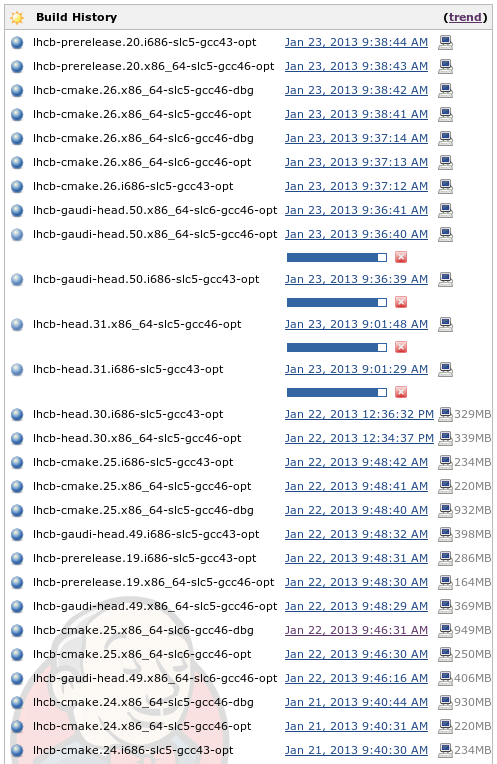
\includegraphics[width=7cm]{jenkins-3}
  \end{center}
  \caption{Jenkins: List of running and recently completed
  \emph{nightly-slot-build} jobs.}
  \label{fig:jenkins-builds}
\end{figure}

The worker jobs are grouped and displayed in the view \emph{Nightly Builds
(workers)} (Figure~\ref{fig:jenkins-workers}), so that they can be easily
monitored and not be confused with the slot jobs.

\begin{figure}
  \begin{center}
    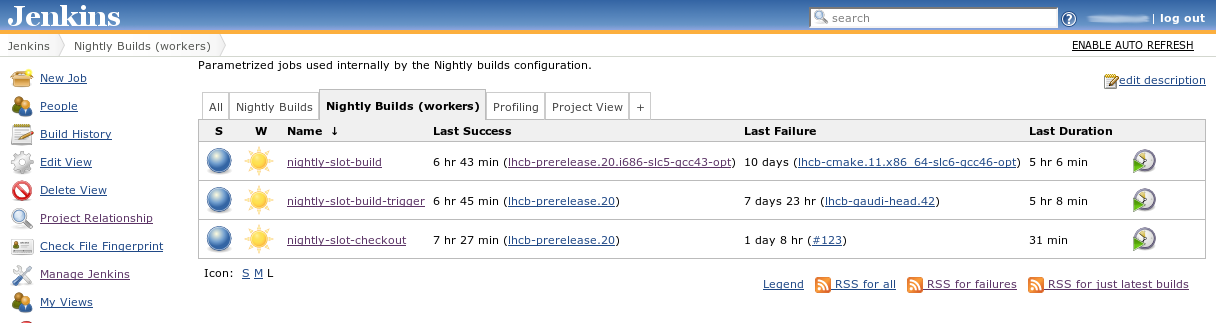
\includegraphics[width=15cm]{jenkins-2}
  \end{center}
  \caption{Jenkins: View of the worker jobs.}
  \label{fig:jenkins-workers}
\end{figure}


\subsubsection{The Slots}
\label{sec:Jenkins:Slots}
To define and build the various slots we use dummy parameterized jobs, one per
slot, named after the slot itself and where the only difference between them is
the name and the default value of the single string parameter
\emph{platforms}\footnote{A string parameter is not very handy to specify the
list of platforms and the
\link{
http://wiki.jenkins-ci.org/display/JENKINS/Extended+Choice+Parameter+plugin}{
Extended Choice Parameter Plugin} could be used to improve usability, but it has
not been tested yet.}, defining the list of platforms the slot is to be built
on.

The configuration of these jobs is relatively simple\footnote{It could be
further simplified by adding one more level of indirection (i.e. another
parameterized worker job), but for the time being it doesn't seem necessary.}.
The build details and artifacts retention policies are the same as the one used
in the configuration of the workers (see \ref{sec:Jenkins:Workers}), for
consistency.  The single string parameter \emph{platforms} has already been
mentioned and is used to define the list of platforms to build when manually
triggering the build, but its default value is what is used for the regular
builds, so, while in the old system the list of platforms to be built was stored
in the configuration file, in the new system is part of the configuration of the
slot job.  Since these are dummy jobs not using CPU, we restrict their execution
to the master node (\emph{Restrict where this project can be run}).  For these
jobs we do not need any source code management.

The build of a slot is triggered via the \emph{Build periodically} configuration
box, which is set to start the builds between 00:00 and 01:00, using the special
schedule \verb|H 0 * * *|, similar to the specification of the Unix
\texttt{cron} command with the special extension \texttt{H} that tells Jenkins
to distribute the builds.  The scheduling can be tuned to build only on some
days as it was possible with some special (and less flexible) settings in the
old configuration.

The build steps for the slots are two simple build triggers, the first one on
\emph{nightly-slot-checkout} and the second one on
\emph{nightly-slot-build-trigger}.  In both cases we pass the following
predefined parameters:
\begin{quote}
\begin{verbatim}
slot=${JOB_NAME}
slot_build_id=${BUILD_NUMBER}
\end{verbatim}
\end{quote}
and we wait for the completion of the triggered job, inheriting the status of
the build.

As for the workers, for easier monitoring, the slot jobs are grouped in a view
called \emph{Nightly Builds} (Figure~\ref{fig:jenkins-slots}).

\begin{figure}
  \begin{center}
    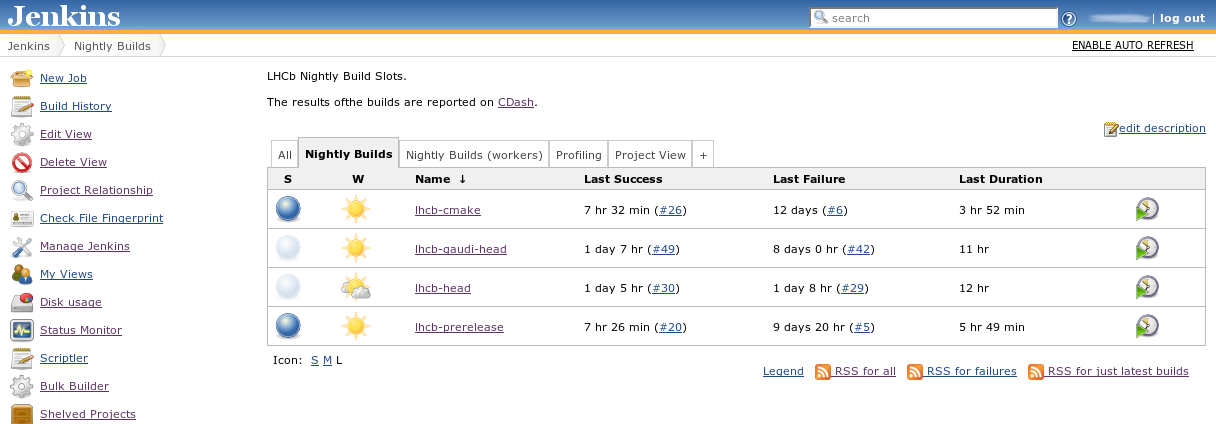
\includegraphics[width=15cm]{jenkins-1}
  \end{center}
  \caption{Jenkins: View of the jobs representing the slots.}
  \label{fig:jenkins-slots}
\end{figure}


\subsubsection{Management Plugins}
\label{sec:Jenkins:Management}
Not strictly needed to run the nightly builds, some plugins have been found very
useful for the simplification of management tasks.
\begin{description}
  \item[Bulk Builder] start several jobs in one go, for example selecting all
the jobs in a view, so that we can re-start all the slots with a few clicks
  \item[Jenkins Disk Usage Plugin] show statistics on the disk space used by the
various builds
  \item[Rebuilder] restart a parameterized build reusing the same parameters,
allowing us to restart the build of a single slot or platform without a new
checkout
  \item[Recipe Plugin] used to store in a file the configuration of a complex
Jenkins setup (jobs, views, plugins) as a \emph{recipe} and import it in another
Jenkins instance, with it we can store the complete configuration of the nightly
build system described in this note
  \item[Shelve Project Plugin] archive projects for possible later use, instead
of deleting them, which is useful to keep a back up copy of some old or
temporary slots
\end{description}
